\documentclass[14pt,twoside]{report}

\usepackage{amsfonts,amsmath,amssymb,stmaryrd,indentfirst}
\usepackage{epsfig,graphicx,times,psfrag}
\usepackage{natbib}
\usepackage{pdfpages,enumerate}% ,enumitem}
 
%%% Rotating Page
\usepackage{pdflscape}
\usepackage{afterpage}
%\usepackage{capt-of}% or use the larger `caption` package
%\usepackage{lipsum}% dummy text


\usepackage[pdftex,bookmarks,colorlinks=true,urlcolor=blue,citecolor=blue]{hyperref}

%\usepackage{fancyhdr} %%%%
%\pagestyle{fancy}%%%%
\pagestyle{empty}
\def\newblock{\hskip .11em plus .33em minus .07em}

\setlength\textwidth      {16.5cm}
\setlength\textheight     {22.0cm}
\setlength\oddsidemargin  {-0.3cm}
\setlength\evensidemargin {-0.3cm}

\setlength\headheight{0in} 
\setlength\topmargin{0.cm}
\setlength\headsep{1.cm}
\setlength\footskip{1.cm}
\setlength\parskip{0pt}

%%%
%%% space between lines
%%%
\renewcommand {\baselinestretch}{1.5}

\begin{document}

%%%
%%% \lipsum % Text before
%%%
\afterpage{%
    \clearpage% Flush earlier floats (otherwise order might not be correct)
    \thispagestyle{empty}% empty page style (?)
    \begin{landscape}% Landscape page
        \centering % Center table
        \vfill
    \end{landscape}
    \clearpage% Flush page
}
\vfill
\clearpage


%%%%%%%
%%%%%%%
%%%%%%%

\begin{center}
  {\Large Review of the Manuscript PNUCENE-D-16-00455 `Analysis the Effects of Error in Movement of Control Rods for WWER-1000 Nuclear Reactor by Developed External Coupling System' by R. Akbari {\it et al.}}
\end{center}

\medskip

The manuscript aims to investigate power transients during xenon oscillations in WWER-1000 reactors. The paper is relatively well-written with a relatively small number of typos and unrevised sentences. A few sentences are confusing and disconnected with no clear objectives (see attached scanned document).  However, the manuscript is insightful although it introduced a limited overview of the main subject areas, e.g., reactor physics design, thermo-hydraulics, neutron-radiation and coupling models.

In fact, from the title I was expecting (a) a comprehensive overview, study and analysis of WWER-1000 reactors with focus on mechanisms (mechanical and neutronics) of control rods (safety control) and methods for fluid - neutronics - nuclear data coupling; (b) an in-depth investigation of the impact of control-rod movements in the neutronics. Unfortunately, none of them was achieved in this manuscript, (a) and (b)  were extremely limited. This manuscript focuses (partially) on (b), and although an extensive quantity of data was generated the analysis was superficial and lacked rigorous structure. In addition, the manuscript fails to clearly state objectives and the novelty of the work -- most of the analysis was conducted before for PWR -- what is the expected difference (of power density output fluctuation due to control rod movement and xenon distribution fluctuations) ? The manuscript however fails to highlight:
  \begin{itemize}
    \item Aim and objectives of the work;
    \item Novelty.
  \end{itemize}
  A few comments:
\begin{enumerate}[(a)] 
%
    \item Several terms were used without and/or before being defined, e.g., BNPP , FSAR, BOC, EOC etc (see attached document);
    \item Several terms in Eqns 1-18 were not defined either in the main text or in the nomenclature table, e.g., $G_{m}$ and $z$ in Eqns. 4-6, $c$ and $\overline{K}_{f}$ in Eqns. 14-15, all terms in Eqns. 16-18 (see attached document);
    \item Some of the thermo-hydraulic equations do not look correct, in particular Eqn. 11. Again I would expect a full explanation of the models used for the thermo-hydraulic model as it would strongly impact on power distribution;
    \item It is seems that the thermal energy equation (Eqn. 6) is parametrised (or non-dimensionalised) and solved semi-analytically through Eqns. 6-8. Is this correct? How is this solution linked with continuity and momentum equation?
    \item Paper's title refers to coupling, however it is not clear how this is actually done. Figures 1, 8-9 attempt to summarise the coupling but it is not really clear how the authors dealt with: (a) time-step size differences between fluid and neutronic models (in the transient calculations), (b) number of energy groups used in the MCNP calculations;
    \item Section 5 (last sentence of the second paragraph) -- comments -re Figs. 4-6: $T_{c,o}$ and $P$ plots do not match at all. Why?
      \item It is clear how Figs. 14-19 prove that control rod movements has limited impact in xenon distribution and power oscillation. In fact, these figures were poorly explained and the conclusions were fully based on the obtained results. 
\end{enumerate}

In summary, the subject of the manuscript is interesting, however the paper still needs to be considerably improved before being considered for publication. The results are insightful and the novelty of the manuscript must be highlighted. 

\medskip
In the scanned copy, PE stands for `Poor English, the authors should consider revise the sentence(s)'.
%%%
%%% Appendix
%%% 
{
  \includepdf[pages=-,fitpaper, angle=0]{./Scan/Scan_PNUCENE_D16_00455.pdf}} 


\clearpage

%%%%%%%
%%%%%%%
%%%%%%%

\begin{center}
  {\Large Review of the Manuscript BJCE-2016-0044.R1 `Challenge Analysis and Schemes Desgn for the CFD Simulation of PWR' by C. Chen {\it et al.}}
\end{center}

\medskip

The manuscript investigates some of the simulations' issues faced by the CFD community worldwide, in particular mesh resolution $\&$ quality and CPU time involving flow analysis in PWRs channels. It is relatively well-written but it contains a large number of typos and unrevised sentences. Several sentences are confusing and disconnected with no clear objectives.  However, the manuscript is insightful although it introduced a limited overview of the main subject area, high-performance computation for PWR simulations. 

In fact, from the title I was expecting a comprehensive study of the main issues on CFD that have large impacts on the nuclear thermo-hydraulic community, e.g., (a) geometric representation (including BC representation of internals); (b) mesh type, resolution and quality (including mesh generation and parallel visualisation of large and complex geometries); (c) discretisation schemes; (d) solver methods (including strategies for efficient HPC and scalability); (e) physical sub-models (e.g., turbulence, heat transfer etc) -- somehow represented in Fig. 21. The present manuscript focuses (partially) on (b) and its potential effects on (a few aspects of) the fluid dynamics. And for the investigation of (b), although an extensive quantity of data was generated the analysis was superficial and lacked rigorous structure. In addition, the manuscript fails to clearly state the novelty of the work -- most of the parametric analysis was conducted before by several authors from the CFD community. A few comments:
\begin{enumerate}[(a)] 
%
    \item {\it Section 2:} all analysis were performed based on a set of numerical simulations using the commercial CFD Fluent. However, the simulation domain (and prescribed geometry and grids), initial and boundary conditions, discretisation and solvers set-up were not properly introduced. There are several published papers reporting error analysis on different grids (mesh type and resolution) and numerical schemes (order of accuracy, upwind/downwind etc).
    \item {\it Section 2.3.1:} last sentence of page 3, `(...) It's always known that structured types are better for data storage and transfer, so the simulation speed of structured mesh is faster and the iteration step number is smaller (...)'. The first part of this sentence has been proved wrong for quite a while (although, one may correctly state that structured grids are easy to implement). Also, what is `iteration step number'? Is it the number of non-linear iterations ? or the (total) number of specific iterations (i.e., for pressure, continuity etc)? or is it something else? 
    \item {\it Section 2.3.1:} What is the effective difference of HP, HP2 and HP3? Is it just the resolution? And what is HP4? Results were shown for this grid but this was not described/introduced.
    \item {\it Section 3.2:} MOC ? 
    \item {\it Section 3.3:} I believe that was the section I could not understand. It is well established within the CFD community that computation time is due to a number of factors, among them (i) mesh type, resolution $\&$ quality; (ii) discretisation schemes; (iii) solver methods and (iv) physics to be solved. Several published CFD studies have demonstrated that most of simulation CPU time are spent on velocity and pressure solvers, which, I believe, the authors parametrised through number of iterations, time-steps and cells. The authors should try to further explain these relationships.
    \item The same is applied to {\it Section 4}.%
\end{enumerate}

In summary, the subject of the manuscript is very relevant, however the paper still needs to be improved before being considered for publication. The results are insightful and the novelty of the manuscript must be highlighted. 

% 

%%%
%%% Appendix
%%%
{
  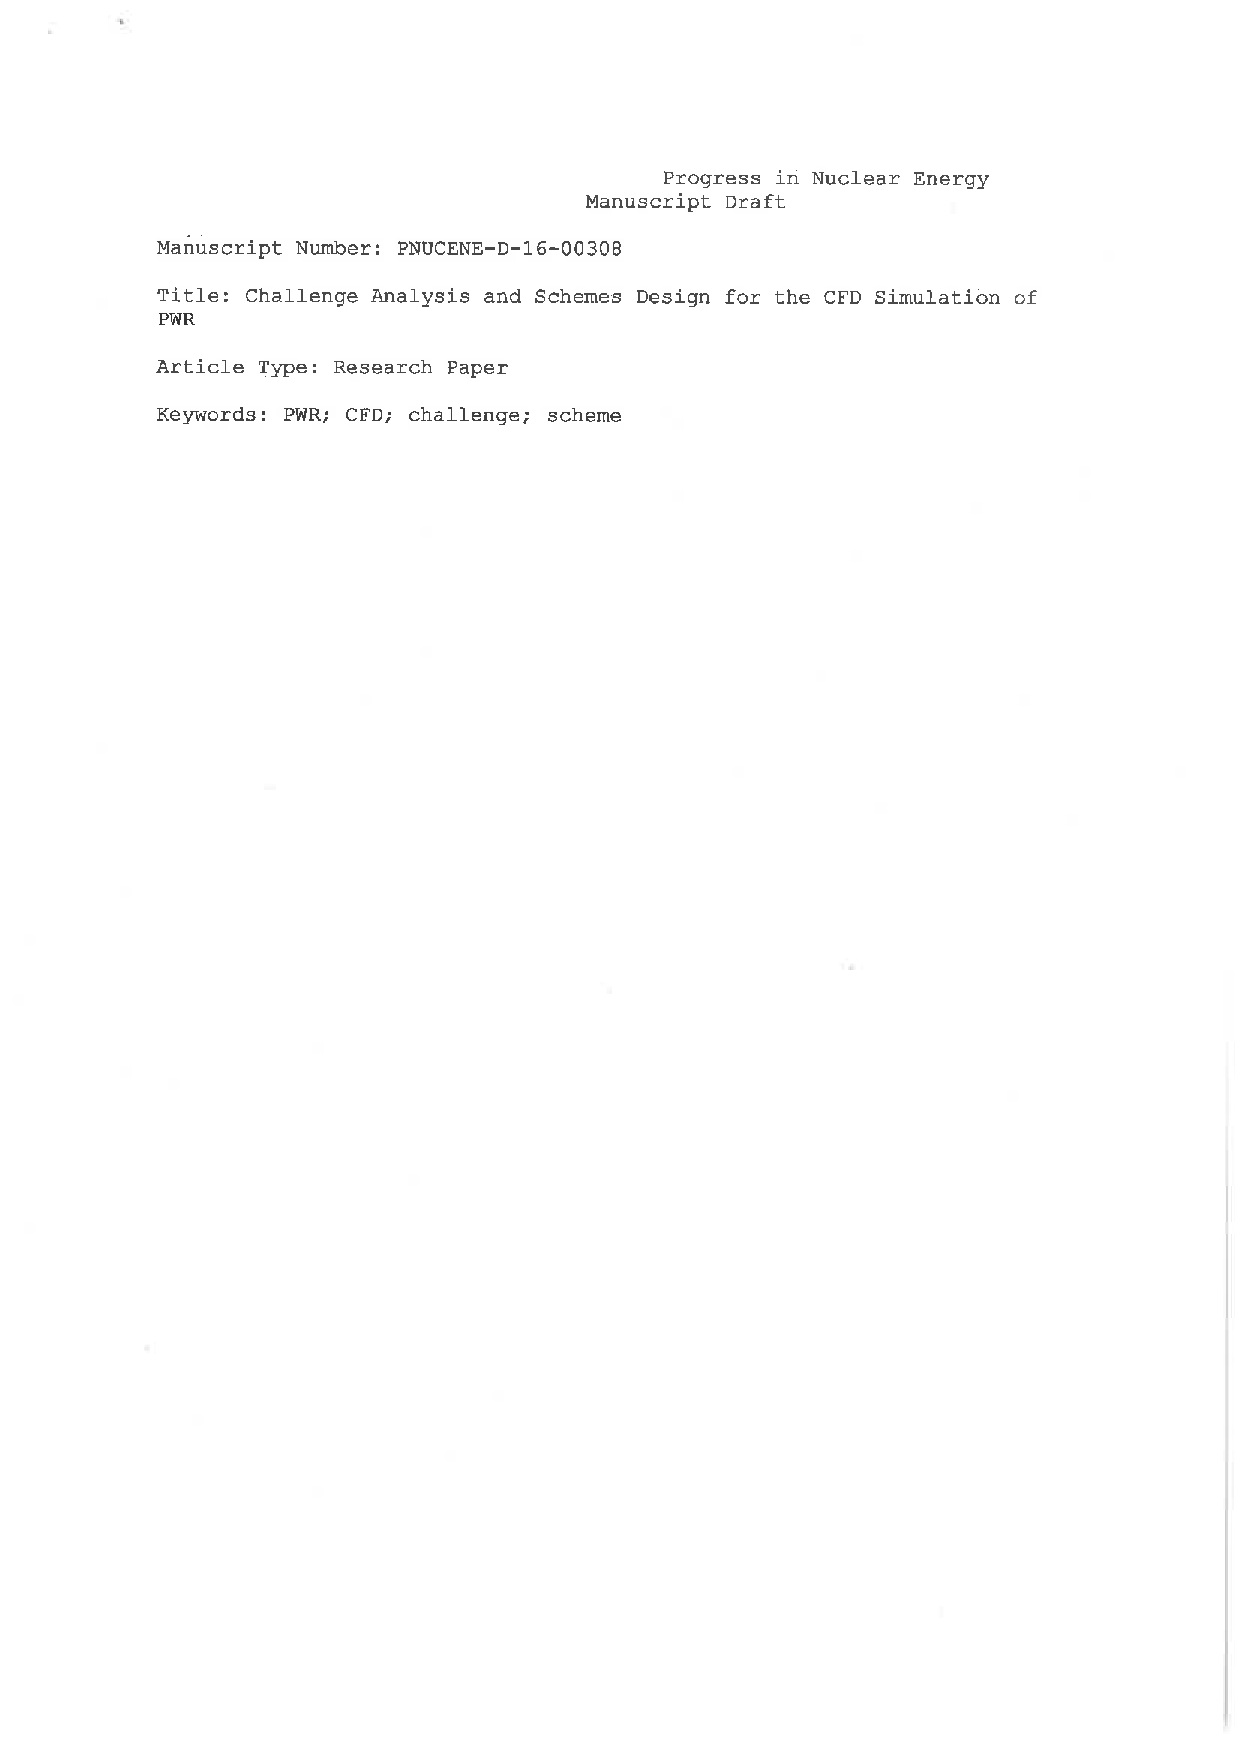
\includepdf[pages=-,fitpaper, angle=0]{./Scan/Scan_PNUCENE-D-16-00308.pdf}} 
  %\includepdf[pages=-,fitpaper, angle=0]{./Scan/Scan_BJCE_2016_0095.pdf}}



\clearpage

%%%%%%%
%%%%%%%
%%%%%%%

\begin{center}
  {\Large Review of the Manuscript BJCE-2016-0044.R1 `Simulation of Species Concentration Distribution in Reactive Flows with Unsteady Boundary Conditions' by A.G. de Oliveira Filho {\it et al.}}
\end{center}

\medskip

The manuscript introduces a novel FEM-based formulation for advection-diffusion-reactive equations and investigates concentration distribution under prescribed boundary conditions. The authors undertook an extensive but comprehensive literature review of a variety of up-to-date models and numerical formulations used in contaminant dispersion in rivers.

The manuscript is relatively well-written with a small number of typos and unrevised sentences (see attached scanned file). A few sentences are confusing and disconnected with no clear objectives. However, the manuscript is comprehensive and introduces an insightful review of the main fundamentals for solving  advection-diffusion-reactive equations.

I am happy that the authors revised the original manuscript, however it still needs revisions before being considered for publication (please see the scanned file). A few comments:
%
\begin{enumerate}[(a)] 
%
\item A few terms need to be defined, e.g, $n$ and $\tau$ in Eqn. 4; $n_{i}$ in Eqn. 7; $B$ in Eqn. 28,  etc
%
\item A paragraph before Eqn. 8: `(...) that advection might effectively occur at the outlet, and {\it said term no longer} represents the (...)'. What do the authors mean with this sentence?
%
\item It clear the FEM-weighted development from Eqn. 2 to Eqn. 11, but how does the velocity magnitude ($U$) appear? This would certainly smear the solution (during the iterative solving procedure), except if $\overline{u}_{x}=\overline{u}_{y}$ which I don't think is the case.
%
\item What is the difference between `pulse injection' and `instantaneous injection'?
%
\item Before Eqn. 17: `(...) in 1-D equation 2 type (...)'. What do the authors mean with {\it 1-D equation 2 type}?
%
\item The manuscript describes the use of a traditional Galerkin method to solve the advection-diffusion-reactive equation (with reaction rate of zeroth-order). What is the solution method used to solve the discretised Eqn. 26?
%
\item I am familiar with natural (NBC) and essential boundary conditions (EBC), but what does MDBC stand for? I believe the readers of BJChE would largely benefit if authors explain these 3 types of boundary conditions. {\bf This is crucial to appreciate the work}.
%
\item Resolution of the figures must be largely improved.
%
\item In the caption of Fig. 4, the simulation was performed with {\it Pe} number of 50, however in the previous paragraph, the authors stated that the {\it Pe} is 100. Which {\it Pe} did the authors used? 
%
\item Last paragraph before Sub-section `2-D Simulation Results' {\bf (ps: appropriated page or section numbering would have greatly improved comments)}: `(...) In this condition, as coarse meshes are adopted (...) MDBC along with sufficiently fine meshes or refined time steps lead to better matching with (...)'. For each {\it Pe} number (Table 1) the authors used mostly one $\Delta x$ (=0.2, which I am assuming is the (maximum) element size) and 1-3 $\Delta t$. Is this enough to support the statement -re mesh refinement and time-step? This would be certainly true if the authors have performed simulations with mesh size and time-steps of different orders of magnitude (e.g., 10$^{-3}\leq\Delta x\leq$ 10$^{-1}$ and 10$^{-4}\leq\Delta x\leq$ 10$^{-1}$).
%
\item First paragraph before Sub-section `2-D Simulation Results': `We observe that the numerical solutions with outlet EBC provide the poorest approximation in all P\'eclet and Damk\"oler numbers considered and that MDBC solutions result in better approximations than NBC in almost all cases'. The authors should give reasons for this statement.
%
\item Figure 6: What is the difference between (A) and (B)?
%
\item Figures 10-12:  I could not understand the meaning of these figures. As stated in the first paragraph of page 23, they were obtained with the same parameters (and I guess the authors refer here to prescribed injection boundary conditions) as in Fig. 9. So why are they so different? I guess the authors imposed spatial-prescribed BCs, is it correct? These figures need to be explained. And why are they important?
%
\end{enumerate}

In summary, the subject of the manuscript is very relevant, however the paper still needs to be improved before being considered for publication. The results are insightful and the novel formulation may introduce an improvement to the accuracy of advection-diffusion-reactive problems under prescribed boundary conditions. 


In the scanned copy,
\begin{itemize}
\item PE: Poor English. The authors should consider revise the sentence(s);
\item SC: Sentence(s) is/are very confusing and do(es) not make any/much sense. The authors should revise the sentence(s).
\item LR: Low resolution (i.e., poor quality) figure.
\end{itemize}


%%%
%%% Appendix
%%%
{
  \includepdf[pages=-,fitpaper, angle=0]{./Scan/Scan_BJCE_2016_0044R1.pdf}}


\clearpage
%%%%%%%
%%%%%%%
%%%%%%%

\begin{center}
  {\Large Review of the Manuscript HYDROL21937 `Accurate Determination of Permeability of Fractured Rocks using Micro-Computed Tomography Images' by H.L. Ramandi {\it et al.}}
\end{center}

\medskip

The manuscript introduces an experimental procedure to assess permeability in fractured rock matrix. The authors undertook a comprehensive literature review of a variety of up-to-date experimental techniques for rock porous network measurement and analysis.

The manuscript is relatively well-written with a small number of typos and unrevised sentences (see attached scanned file). A few sentences are confusing and disconnected with no clear objectives. However, the manuscript is comprehensive and introduces an insightful review of the main fundamentals on the main issues of rock characterisation -re matrix permeability.

The manuscript however fails to highlight:
  \begin{itemize}
    \item Aim and objectives of the work;
    \item Novelty.
  \end{itemize}
A few comments:
\begin{enumerate}[(a)] 
%
\item {\it Abstract} and {\it Section 1:} authors should clearly indicate the main aim and objectives of the work;
%
\item What are the main advantages of the techniques introduced by the authors in comparison with the existing ones? For example, Table 2 benchmarks the introduced technique with distinct sub-scale resolutions against `experimental permeability', how does the technique compares with others?  
%
\item {\it Last paragraph of Section 2:} `(...) Permeability prediction is obtained based on the finite volume solution of the Stokes equation (...) $\mu$ is the fluid viscosity.' What do the authors mean with this sentence? How can the Stoke equation be used to calculate permeability?
%
\end{enumerate}
% 
I have 2 main concerns about this manuscript that the authors must address,
\begin{enumerate}[(i)]
\item An appropriate validation of the introduced technique;
\item The authors must clearly state the novelty that the manuscript addresses.
\end{enumerate}

In summary, the subject of the manuscript is very relevant, however the paper still needs to be improved before being considered for publication. The results are insightful and the novel technique may introduce an improvement to the  accuracy of current permeability measurements. 


%%%
%%% Appendix
%%%
{
  \includepdf[pages=-,fitpaper, angle=0]{./Scan/Scan_Hydrol21937.pdf}} 
  %\includepdf[pages=-,fitpaper, angle=0]{./Scan/Scan_BJCE_2016_0095.pdf}}



\clearpage


%%%%%%%
%%%%%%%
%%%%%%%

\begin{center}
  {\Large Review of the Manuscript BJCE-2016-0095 `Mathematical Model of the Temperature and the Concentration Profiles of an Industrial Rotary Kiln used in Clinker Production' by D.C.Q. Rodrigues {\it et al.}}
\end{center}

\medskip

The manuscript introduces a mathematical procedure to model gas and solid flows in rotary kiln. The authors undertook a comprehensive, but limited, literature review of the current problems in the clinker production. The manuscript briefly described the main conservation and constitutive equations used in the industry-standard model by {\it Spang (1972)} and the modification suggested by the author. Simulations were performed in a 2-D system.

The manuscript is relatively well-written with a small number of typos and unrevised sentences. A few sentences are confusing and disconnected with no clear objectives.  However, the manuscript is comprehensive although it introduced a very superficial literature review on the main subject area, clinker production. In fact, as the manuscript mainly focuses on simulations' results, I would expect a short literature review on any (if not all) of the subject that are relevant to the clinker production field, e.g., heat and mass transfer mechanisms, chemical kinetics and thermodynamics, multiphase (solid-fluid) flows, etc (e.g., Ngako {\it et al.}, 2015, Powder Technology 271:221-227; Atmaca $\&$ Yumrutas, 2014, Applied Thermal Engineering 66:435-444; Sogut {\it et al.}, 2010, Applied Thermal Engineering 30:817-825 etc). 

The manuscript fails to clearly state the novelty of the work -- the authors modified the existing Spang model, but have not explicitly explained how the changes impacted in the solution or why these changes were performed. A few comments:
\begin{enumerate}[(a)] 
%
\item The aim of the paper is to introduce a new model of rotary kiln for clinker production. The model is based on the existing Spang model, in which the main equations are available in the Appendix. However, the authors must explain the existing model (conservation + constitutive equations + boundary conditions and main assumptions + simplifications) before introducing the modifications (with the appropriate reasoninig for those changes). 
%
\item In page 4 (lines 10-11): `(...) The results qualitatively describe the behaviour of kilns, but the steady state was not reached.' Why not? And what about quantitative behaviour of the Spang model?
%
\item Several terms in the equations (in the Appendix) are not in the list of symbols.
%
\item Equations 13-15 describe the thermal energy balance of gas, solid phases and the wall (I am not sure if the existence of Eqn. 15 is correct). Why isn't there any time-term in the gas-equation original model (Eqn. 13)? I understand that this is the authors' contribution for the new model, but it is difficult to understand how someone would have solved the transient for the solid phase (and the wall as well) but not for the gas phase. What is Spang's assumption? 
%
\item The model introduced by the authors replaced the thermal energy source term, $q_{f}$ (Eqn. 17, flame equation) by discrete values obtained from field data (page 5, lines 8-12). Why was this necessary? What is the discrepancy between discrete $q_{f}$ (industry-based) and the obtained from Eqn. 17?
%
\item Second paragraph of page 5 (lines 33-44): `(...) final composition of the clinker obtained in the simulation was similar to the actual values obtained in the cement industry (Table 5)'. What is the criteria to assess this {\it similarity}? Data in Table 5 for field and simulation data do not seem to match, a simple error analysis revealed discrepancies ranging from 17$\%$ to 52$\%$.
%
\item The manuscript is about a new mathematical model, but the description of the model and the numerical methods/schemes used to solve the set of equations were very poor.
%
\item Figures 6-9 describe sensitivity analysis of the simulation, i.e., what is the impact of changes in gas/solid inlet velocity in both temperature and concentration (gas and solid phases) fields. The results are interesting but disappointingly there is no analysis of the results.
%
\item I guess the main problem in this manuscript is the lack validation of the new model. No comparison (apart from Table 5, commented above) with either Spang model, experiments or field data is quantitatively (and/or statistically) introduced.
%
\end{enumerate}

I have 4 main concerns about this manuscript that the authors must address,
\begin{enumerate}[(i)]
\item A thorough description of the model;
\item An in-depth analysis of the solutions presented;
\item An appropriate validation of the introduced model;
\item The authors must clearly state the novelty that the manuscript addresses.
\end{enumerate}

In summary, the subject of the manuscript is very relevant, however the paper still needs to be largely improved before being considered for publication. The results, although interesting (but poorly discussed), does not bring much novelty to the field -- or at least the authors failed to explicitly demonstrate it. 


%%%
%%% Appendix
%%%
{
  \includepdf[pages=-,fitpaper, angle=0]{./Scan/Scan_BJCE_2016_0095.pdf}}



\clearpage

%%%%%%%
%%%%%%%
%%%%%%%


\begin{center}
  {\Large Review of the Manuscript CAM-D-15-02454 `Mixed Volume Element Combined with Characteristic Mixed Finite Volume Element Method for Oil-Water Two-Phase Displacement Problem' by Yuan {\it et al.}}
\end{center}

\medskip

The manuscript describes a hybrid FEM-FVM-Characteristic method to solve the elliptic coupled mass balance and force balanced equations representing the (Darcy) flows in porous media. The authors undertook a comprehensive literature review of the main fluid methods with focus on mixed FEM.

The manuscript is relatively well-written with a small number of typos and unrevised sentences. A few sentences are confusing and disconnected with no clear objectives. However, the manuscript is comprehensive and introduces an insightful review of the main fundamentals on FEM-based methods for porous media flows. 

The manuscript however fails to highlight:
  \begin{itemize}
    \item Aims and objectives of the work
    \item Novelty.
  \end{itemize}
A few comments:
\begin{enumerate}[(a)] 
%
\item {\it Abstract} and {\it Section 1:} authors should include aims/objectives of the work;
%
\item {\it Section 2:} Are $\alpha_{i}$ (with $i$ = 1,2) arbitrary constants? Also (page 5), $D_{j}$ and $d_{j}$ were used before being defined. I am not if the former is a component of the diffusion coefficient (Eqn. 1.2) or a linear-operator.
%
\item {\it Section 5:} Validation undertook for the method introduced in {\it Section 3} seems very limited. And how does it compare (accuracy) with Arbogast $\&$ Wheeler? Analysis of the solutions in this section were superficial.
%
\end{enumerate}
I have 3 main concerns about this manuscript that the authors should address,
\begin{enumerate}[(i)]
\item An in-depth analysis of the numerical solutions presented in Figs. 2-9;
\item The authors must clearly state the novelty that the manuscript addresses.
\end{enumerate}

In summary, the subject of the manuscript is very relevant, however the paper still needs to be improved before being considered for publication. The results, although interesting (but poorly discussed), does not bring much novelty to the field -- or at least the authors failed to explicitly demonstrate it. 

\clearpage

%%%%%%%
%%%%%%%
%%%%%%%


\begin{center}
  {\Large Review of the Manuscript POWTEC-D-15-01601 `Discrete Element Modelling of Sediment Falling in Water' by Wang $\&$ Tan}
\end{center}

\medskip

The manuscript describes a set of numerical simulations of granular particles falling in fluid at rest (thus no imposed fluid velocities into the particles). The authors undertook a brief, but comprehensive, literature review of the main computational tecnologies on granular flows with focus on continuum (mainly CFD) and discrete models (mainly DEM) currently used. The main aim of the paper is to investigate (and validate) momentum transfer forces and formulations (Table 2) in the DEM framework. Simulations were performed usin g the open-source LAMMPS model and compared against lab experiments.

The manuscript is relatively well-written with a small number of typos and unrevised sentences. A few sentences are confusing and disconnected with no clear objectives. However, the manuscript is comprehensive and introduces an insightful (but superficial) review of fluid-solid mometum transfer models. The manuscript briefly reviewed the main equations for drag and added mass forces, and briefly summarises the Stokeslet disturbance formulation. 

There were other publications that extensively investigated the impact of drag and added mass forces in granular flows and, in particular, in fluidisation in both continuum and discrete models. Momentum transfer models based on solid concentration (volume fraction) and the impact of particles' motion on the surrounding fluid flows have been largely studied by the granular CFD community. A few comments:
\begin{enumerate}[(a)] 
%
\item Page 2: `(...) and complex fluid systems, that CFD results are generally non-disputed (...)': Not really, CFD, as any model, relies on extensive software and model quality assurance (verification and validation); 
%
\item Page 7: `(...) which are related to the particles material properties (see Table 1)': I believe the authors have not included this table;
%
\item Second paragraph of page 16: The authors described the numerical solutions (Fig. 2) but no analysis was conducted;
%
\item First paragraph of page 18: Why do the models behave in such way? 
%
\end{enumerate}
I have 3 main concerns about this manuscript that the authors should address,
\begin{enumerate}[(i)]
\item An in-depth analysis of the numerical solutions presented in Figs. 2-5;
\item Comparison against experimental data is very superficial and lacks a proper statistical analysis;
\item The authors must clearly state the novelty that the manuscript addresses.
\end{enumerate}

In summary, the subject of the manuscript is very relevant, however the paper still needs to be improved before being considered for publication. The results, although interesting (but poorly discussed), does not bring much novelty to the field -- or at least the authors failed to explicitly demonstrate it. 

\clearpage


%%%%%%%
%%%%%%%
%%%%%%%


\begin{center}
  {\Large Review of the Manuscript PNUCENE-D-15-00347 `Evaluation the effects of steam state equation, spray and multi-cell subdivisions on Containment pressurization modelling in a LB-LOCA' by Noori-Kalkhoran $\&$ Matajy-Kojouri}
\end{center}

\medskip

The manuscript summarises a global system methodology to assess a few safety parameters during a LB-LOCA event. It briefly describes two strategies to model heat flux and pressure oscillations in reactor containments: (a) single (or one-volume) cell and, (b) multi-cell models. Both methods assume mass conservation in a cell (or across cells) and attempt to calculate heat flux and phase change with imposed initial conditions (severe accident condition).

The manuscript is relatively well-written with a number of typos and unrevised sentences (see the attached scanned document). A few sentences are confusing and disconnected with no clear objectives. However, the manuscript is comprehensive and introduces an insightful (but superficial) review of the methods used to model heat and mass flux (thermo-hydraulic) in reactor containments.  I would expect a short literature review on the main subject areas of the paper (e.g., transient heat transfer with phase change, volume system models, etc). The manuscript also briefly reviewed the main equations used to model these phenomena. In fact, my main concern is that the equations were not fully explained, i.e., main constraints and range of applicability. And also, it is not clear if the authors developed the models using these equations or if they used an industry-standard system code/software. A few comments:
\begin{enumerate}[(a)] 
%
\item Several terms use different symbols throughout the manuscript, making the reading more difficult, e.g., specific enthalpy ($i$, $h$ and $H$), mass flow ($\dot{M}$ and $G$), spray (subscripts $sp$ and $\text{\it spray}$). Also some indices have changed throughout the sections, e.g., $k$ and $K$ from Eqn. 42 onwards;
%
\item The authors should consider adding more descriptive (and self-contained) figure captions;
%
\item Some terms were used before being defined, e.g., IRIS, FSAR, LB-LOCA etc;
%
\item Section 2.1 was very confusing and not well explained -re the validity of the equations;
%
\item Section 2.2:
   \begin{enumerate}[(i)]
      \item Eqn. 9 should read as,
        \begin{displaymath} 
           M_{D}\left(t+\Delta t\right) = \int\limits_{t}^{t+\Delta t} \left(\dot{M}_{DB}-\dot{M}_{SC}-\dot{M}_{WC}\right)dt + M_{D}(t)
        \end{displaymath}
      \item The term `{\it flash}' in the first line of this section (also throughout the text), does it refer to isothermal (or isenthalpic) flash or just to fluid flow into/out of the containment?
      \item In Eqn. 12, how are $P_{\text{max}}$ and $P_{\text{min}}$ calculated/obtained? 
   \end{enumerate}
%
\item Equations of state for the water/steam-air system are briefly described in Section 2.3.1. Why do the authors assumed that air should behave as an ideal gas? Properties of saturated water and superheated steam were obtained from water/steam thermodynamic tables. Are these tabulated or calculated `{\it on the fly}' (i.e., online)?
%
\item In Section 3.1, it seems that the author assume all fluids incompressible (Eqn 27), why?
%
\item Section 5:
   \begin{enumerate}[(i)]
      \item Could the authors explain the DECL accident scenario? I guess this would be useful for the PNE readers. Why was this accident scenario chosen?
      \item Results were shown in Figs 9-18 (with and without spray). However no reason was given for the best performance of the multi-cells system (in comparison with the single-cell). Also, why is there large discrepancy (pressure and temperature fields) between FSAR and the calculated models in the beginning of the transient?  
   \end{enumerate}   
%
\end{enumerate}

In summary, the subject of the manuscript is very relevant for nuclear technology community, however the paper still needs to be largely improved before being considered for publication. The results, although interesting (but poorly described and discussed), does not bring much novelty to the field -- or at least the authors failed to explicitly demonstrate it. 



In the scanned copy,
\begin{itemize}
\item PE: Poor English. The authors should consider revise the sentence(s);
\item SC: Sentence(s) is/are very confusing and do(es) not make any/much sense. The authors should revise the sentence(s).
\end{itemize}


%%%
%%% Appendix
%%%
{
  \includepdf[pages=-,fitpaper, angle=0]{./Scan/Scan_PNUCENE-D-15-00347.pdf}

%%%
%%% \lipsum % Text before
%%%
\afterpage{%
    \clearpage% Flush earlier floats (otherwise order might not be correct)
    \thispagestyle{empty}% empty page style (?)
    \begin{landscape}% Landscape page
        \centering % Center table
           \Huge{2015}
        \vfill
    \end{landscape}
    \clearpage% Flush page
}
\vfill
\clearpage

%%%%%%%
%%%%%%%
%%%%%%%


\begin{center}
  {\Large Review of the Manuscript AMC-D-15-01974 `A New Metropolis Optimization Method, the Cross-Section Particle Collision Algorithm' by Sacco $\&$ Henderson}
\end{center}

\medskip

The manuscript introduces a modified PCA optimisation algorithm, based on the phase-space search-acceptance strategy within the scattering stage. The performance of the CSPCA algorithm was assessed through 5 optimisation test-case problems.

 
The manuscript is well-written with a small number of typos and unrevised sentences (see the attached scanned document). A few sentences are confusing and disconnected with no clear objectives. 

The method and benchmarks introduced in the manuscript are very challenging, however reading the manuscript is difficult to identify the authors' original contribution. It is clear that CSPCA is a more complex algorithm than the original PCA -- and also more efficient for the set of non-linear benchmark test-cases. The weighted acceptance Monte Carlo-based criteria has some resemblance with the cross-section generation, so how important the scattering stage is within the PCA family of methods? The overall performance of the CSPCA, highlighted in Tables 1-4, does not seem to differ that much from the traditional PCA, if we consider both SR and average NFE. Why? May it be a problem in the scattering stage implementation (maybe in the way the probabilistic function is defined)?  

%%%
%%% Appendix
%%%
{
  \includepdf[pages=-,fitpaper, angle=0]{./Scan/Scan_AMC-D-15-01974_Review.pdf}


%%%
%%% \lipsum % Text before
%%%
\afterpage{%
    \clearpage% Flush earlier floats (otherwise order might not be correct)
    \thispagestyle{empty}% empty page style (?)
    \begin{landscape}% Landscape page
        \centering % Center table
        \vfill
    \end{landscape}
    \clearpage% Flush page
}
\vfill
\clearpage




\begin{center}
{\Large Review of the Manuscript ADWR-15-232 `An Implicit Numerical Model for Multicomponent Compressible Two-Phase Flow in Porous Media' by A. Zidane and A. Firoozabadi}
\end{center}

\medskip

The manuscript describes an implicit model for compressible multiphase and multi-componet flows in porous media. Numerical simulations were performed using the new model approach with initial comparison against commercial model software under a number conditions. 

The manuscript is relatively well-written with a small number of typos and unrevised sentences (see the attached scanned document). A few sentences are confusing and disconnected with no clear objectives. However, the manuscript is comprehensive and introduces an insightful (although superficial) literature review on the main subject areas. In fact, as the manuscript mainly focuses on an implicit formulation for compressible flows, I would expect a short literature review on this subject. There is a good number of manuscripts on the fluid dynamics open literature on compressible (including shock-capturing and high-order accurate schemes), multi-component and implicit-/explicit-DG formulations. A few comments:
\begin{enumerate}[(a)] 
%
\item I understand that the authors do not want to reveal the commercial flow simulator software used for model validation, referred as CM-1/2/3. However, in order to properly appreciate the validation exercise it is necessary to know some info of this set of software, are they FEM- or FVM-based (or hybrid, CVFEM, EbFVM)? What sort of element/volume and formulation (spatial- and time-discretisation) they use?
%
\item In Eqn. 7, what does $\beta$ represent? Does it refer to the remaining phases?
%
\item The last two sentences of page 11: `The coefficient $c_{\alpha}x_{i,\alpha}$, (...) without considering higher-order spatial approximations. This is due to the fact that the pressure is a smooth function of space in the scope of this work'. What do the authors mean here? Pressure and phase velocities are coupled via the Darcy equation (Eqn. 3), thus a similar high-order approximation should be used in both velocity and pressure fields.
%
\item In the last sentence of pages 11-12, the authors stated that the upwind scheme used in the scalar transport equation can not be used in the pressure equation. Why not? So what is done in the proposed formulation?
%
\item A major issue in numerical modelling of compressible multiphase flows is the transition between incompressible (e.g., liquids) and compressible fluids due to the strong non-linear coupling between densities and pressure (i.e., speed of sound in fluids $\left(\eta^{2}=\left[\frac{\partial p}{\partial \rho}\right]\right)$. How does the formulation treat such discontinuities?
%
\item Simulations were performed in Section 4, where numerical solutions obtained from the formulation were qualitatively validated against commercial models (cross-code validation) and against an explicit DG model. The path for validation chosen by the authors seems consistent with much of the porous media open literature, however I wonder why didn't the authors try to quantitatively validate the model against simple 1D analytic solution (3-4 components) and then qualitatively validate against other models.
%
\item Last sentence of page 13, does the average number of Newton iteration refer to the convergence of the VLE sub-model (based on the PR EOS) or the actual Picard method (or non-linear iteration) of the whole set of conservative equations (pressure, saturation and compositional)? I believe the authors refers to the later, in this case, in the formulation are all fields are lumped together and solved in a single operation or in field-based stages (e.g., velocity-pressure $\rightarrow$ saturation $\rightarrow$ mass/mole fraction etc).
%
\end{enumerate}

%%%
%%% Appendix
%%%
{
  \includepdf[pages=-,fitpaper, angle=0]{./Scan/Scan_ADWR-15-232_Review.pdf}
}


%%%
%%% \lipsum % Text before
%%%
\afterpage{%
    \clearpage% Flush earlier floats (otherwise order might not be correct)
    \thispagestyle{empty}% empty page style (?)
    \begin{landscape}% Landscape page
        \centering % Center table
        \vfill
    \end{landscape}
    \clearpage% Flush page
}
\vfill
\clearpage

%%%%%%%
%%%%%%%
%%%%%%%


\begin{center}
{\Large Review of the Manuscript PNUCENE-D-15-00085 $\lq$A Comparative Study of Pool and Dry-Cask Storage System PRAs for Spent Nuclear Fuel' by {\it S. Zhang et al.}}
\end{center}

\medskip

The manuscript describes the procedure for preliminary risk assessment in nuclear fuel storage systems. The work is based on pilot studies in two nuclear power plants in China operating with distinct storage systems: pool and dry-cask. The paper is well-written with a small number of typos, a few sentences are confusing and disconnected with no clear objectives. 

In general, the manuscript is comprehensive and introduces best-practive procedures for PRA analysis for spent nuclear fuel storage.  However, my main concern is that there is no clear indication of neither scientific objectives of the paper nor novelties that the authors are bringing. In fact, the paper focuses on the main conclusions of PRA analysis, without any indication of a new methodology.  


%%%
%%% \lipsum % Text before
%%%
\afterpage{%
    \clearpage% Flush earlier floats (otherwise order might not be correct)
    \thispagestyle{empty}% empty page style (?)
    \begin{landscape}% Landscape page
        \centering % Center table
        \vfill
    \end{landscape}
    \clearpage% Flush page
}
\vfill
\clearpage

%%%%%%%
%%%%%%%
%%%%%%%

\begin{center}
  {\Large Review of the Manuscript BJCE-2015-0011 $\lq$3D Compositional Reservoir Simulation in Conjunction with Unstructured Grids' by Ara\'ujo {\it et al.}}
\end{center}

\medskip

The manuscript aims to demonstrate the functionalities of a compositional model formulation embedded in the UTCOMP flow simulator. The model is based on the element-based finite volume method (EbFVM) and benchmarks were performed with a number of element/cell types. The authors presented a brief (and limited) literature review on the current state-of-the-art of flow simulator methods and formulations and performed a set of numerical simulations. 

The manuscript is relatively well-written with a small number of typos and unrevised sentences (see the attached scanned document). A few sentences are very confusing and disconnected with no clear objectives. The method and benchmarks introduced in the manuscript are very interesting, however reading the manuscript is difficult to identify the authors' original contribution. What novelties do the manuscript bring? A few notes/questions:
\begin{enumerate}
%
\item Some terms were used before being defined, e.g., $\lq$PEBI' in the Abstract;
\item Page 4 (lines 34-47): one of the main features in the model is the use of the EbFVM instead of more traditional (for flow simulators) FEM, FDM and CVFEM. However, no specific explanation of the method is given, except $\lq$(...) The main difference between CVFEM and EbFVM techniques lies in the assumption of multiphase/multicomponent flow of the EbFVM approach in order to obtain the approximated solution (...)'. It is not clear the difference between the methods, surely neither FEM nor CVFEM are not bounded by single/multi-phase/component nature of flows. Thus I guess the author possibly meant some scalar field conservation aspect;
\item Indices in Eqn 1 and the text following it seems to be messed up; 
\item Is Eqn 2 correct? A quick dimension analysis indicates a mismatch -re $\gamma_{i}D$ term, assuming that $\gamma$ is molar weight (or molar mass, g/mol) and $D$ is reservoir depth (m);
\item Does the formulation take into account anisotropy of permeability tensors? In the tables, the diagonal components of permeability are given, thus I am assuming the synthetic geological formation is rather homogeneous, is it correct?
\item Was there any study on the convergence test performed for the formulation presented in the manuscript? 
%
\end{enumerate}
In the scanned copy,
\begin{itemize}
\item PE: Poor English. The authors should consider revise the sentence(s);
\item SC: Sentence(s) is/are very confusing and do(es) not make any/much sense. The authors should revise the sentence(s).
\end{itemize}

%%%
%%% Appendix
%%%
{
  \includepdf[pages=-,fitpaper, angle=0]{./Scan/Scan_BJCE_2015-0011.pdf}


%%%
%%% \lipsum % Text before
%%%
\afterpage{%
    \clearpage% Flush earlier floats (otherwise order might not be correct)
    \thispagestyle{empty}% empty page style (?)
    \begin{landscape}% Landscape page
        \centering % Center table
        \vfill
    \end{landscape}
    \clearpage% Flush page
}
\vfill
\clearpage

%%%%%%%
%%%%%%%
%%%%%%%


\begin{center}
{\Large Review of the Manuscript PNUCENE-D-14-00301 $\lq$CFD Study of an air-water flow inside helically coiled pipes' by {\it M. Colombo et al.}}
\end{center}

\medskip

The manuscript investigates multiphase (air-water) flow dynamics in helical pipes with a two-fluids model formulation.  Numerical simulations were performed using the FLUENT model software using a number of mesh grids and flow conditions. 

The manuscript is relatively well-written with a small number of typos and unrevised sentences (see the attached scanned document). A few sentences are confusing and disconnected with no clear objectives. However, the manuscript is comprehensive and introduces an insightful although very superficial literature review on the main subject areas. In fact, as the manuscript mainly focuses on multi-fluid dynamics in confined domains, I would expect a short literature review on this subject. There is a good number of manuscripts on the nuclear and non-nuclear open literature on both internal and external (single- and multiphase) flows and heat transfer in and around helically coiled pipes (see Y.J. Chung 2013 and 2014, Buchan 2012, all in {\it Annals}). A few comments:
\begin{enumerate}[(a)]
%
\item  The main objective of the paper (lines 27-38 of the {\it Abstract}) is to investigate flow dynamic parameters (pressure drop and void volume fraction) in helicoidal pipes. As these parameters are strongly dependent on the geometry (e.g., pipe diameter, coil pitch and curvature etc) and thermo-physical properties of the fluid (e.g., fluids' density, viscosity, velocity) I would suggest the authors to include a schematic of the helicoidal pipes. This would help understand the system the authors are simulating.
%
\item Also, as coil pitch and curvature play  crucial roles in the flow dynamics (in particular bubble formation and growth), I would expect an in-depth sensitivity analysis of these parameters.
%
\item Most of plots shown in the manuscript are functions of the {\it $\lq$quality'}, $x$. The authors have not defined this term. I am aware that flow quality is often associated with quantity of vapour phase in the two phases dome region, 
\begin{displaymath}
x_{i} = \frac{\Psi_{i} - \Psi_{\text{liq}}}{\Psi_{\text{vap}}-\Psi_{\text{liq}}}
\end{displaymath}
where $\Psi$ is any extensive thermodynamic property (e.g., specific enthalpy, entropy etc) and $i$ refers to flow conditions (i.e., pressure and temperature). Thus, in Figs. 1 and 2 (air and water experimental flow), which component does the quality refer to ? I have not read the reference paper, but I would guess that the quality refers to the amount of air in the mixture (assuming that air does not get dissolved in water), therefore the authors actually refer to the gas volume fraction. The authors should make it clear.
%
\item Last sentence of the first paragraph of Section 2. Why did the authors choose this specific experimental data set to validate their model/simulations?
%
\item In Section 3, the authors summarised the numerical options used in the simulations. As some of the readers (including myself) are not familiar with ANSYS FLUENT framework I would really suggest the authors to describe in (some) depth the methods, discretisation, schemes and solvers options used by the authors as this may explain the reason why some of the results presented seems to be slightly dissipative. 
%
\item Also, as the study focuses on pressure drop in the gas-liquid mixture (and the relationship with drag), authors should shown the equations used to represent drag and bulk density and viscosity linearisation, as they may play a significant role in the momentum conservation.
%
\item Figures 3,13 and 17 are low resolution (poor quality) and should be improved.
%
\item In Section 4, the authors performed a grid sensitivity analysis that led to the choice of mesh used in the remaining of the work. However, their procedure to choose the mesh is very random and does not make any sense. Three distinct mesh grids, three distinct inlet velocities for the gas and liquid phases and three distinct initial gas volume fraction. The resulting pressure drop {\it versus} number of cross-section cells did not shown any convergence that would indicate a grid independent solution. The authors should ensure that the mesh used in the simulations is the optimal mesh, i.e., solution is not dependent on the grid. 
%
\item Section 5: 
\begin{enumerate}[(i)]
%
\item 2$^{\text{nd}}$ paragraph: Bubble / droplet diameter are not imposed in CFD calculations (this is clear from the set of conservative equations you are solving for, where volume fraction of phases will increase/decrease depending on the flow but are also naturally constraint), however they are used as threshold in the constitutive equations to induce bubble formation, drag increase (Eqn. 5) etc.
%
\item Are the profile figures time-averaged and time-snapshots fields? I would guess the later, if this is the case, the authors should indicate the position in the helical coil and the time-stamp.
%
\item As this section investigate the influence of $d_{p}$ in the dynamics, and more specifically in the inter-phase momentum transfer, I would expect a more thorough discussion on the used drag formulation instead of just a set of simulations with different initial conditions. I believe the authors are not resolving the inter-phase momentum transfer, but rather relying on drag correlations -- so which correlation were used in the simulations?
%
\end{enumerate}
%
\item Section 6: A few CFD models treat the centrifugal term as part of gravitational term but implicitly embedded into the pressure term in the momentum equation. How is centrifugal force treated in Fluent? I would guess that this is part of the rotational reference framework in Fluent, is it correct? Please explain.
%
\item Section 7.1: The authors should explain (preferentially with the relevant equations) the wall function and the enhanced wall treatment formulations in the Fluent model. Also, was the new finer grid close to the walls regular- or exponential-based?  
%
\end{enumerate}


%%%
%%% Appendix
%%%
{
  \includepdf[pages=-,fitpaper, angle=0]{./Scan/Scan_PNUCENE_D14_00301.pdf}
}

%%%
%%% \lipsum % Text before
%%%
\afterpage{%
    \clearpage% Flush earlier floats (otherwise order might not be correct)
    \thispagestyle{empty}% empty page style (?)
    \begin{landscape}% Landscape page
        \centering % Center table
        \vfill
    \end{landscape}
    \clearpage% Flush page
}
\vfill
\clearpage

%%%%%%%
%%%%%%%
%%%%%%%



   
\end{document}
